\documentclass{oblivoir}
\usepackage{amsmath,amssymb,amsthm,kotex,mdframed,paralist,graphicx,tabu,mdframed}
\newcommand\pb[1]{\ensuremath{\fbox{\phantom{#1}}}}

\usepackage{fapapersize}
\usefapapersize{210mm,297mm,40mm,40mm,30mm,30mm}

\newcounter{num}
\newcommand\prob[1]
{\bigskip\par\noindent\stepcounter{num} \textbf{문제 \thenum) #1}\par\noindent}
\newcommand\ans[1]
{\par{\raggedleft\textbf{답 : #1}
\par}\bigskip\bigskip}

\usepackage{tabto,pifont}
\TabPositions{0.2\textwidth,0.4\textwidth,0.6\textwidth,0.8\textwidth}
\newcommand\tabb[5]{\par\noindent
\ding{172}\:{\ensuremath{#1}}
\tab\ding{173}\:\:{\ensuremath{#2}}
\tab\ding{174}\:\:{\ensuremath{#3}}
\tab\ding{175}\:\:{\ensuremath{#4}}
\tab\ding{176}\:\:{\ensuremath{#5}}}

%%%
\begin{document}

%%
\section*{EBS 올림포스 문제들}

%
\prob{}
그림과 같이 중심이 \(O\)이고 반지름의 길이가 \(50\) m인 반원 모양의 땅에 넓이가 \(2400\) m\(^2\)인 직사각형 모양의 땅이 접해있다.
이 곳에 그림과 같이 \(A\), \(B\), \(C\), \(D\), \(E\)지점을 지나는 도로를 만들려고 할 때, 이 도로의 길이의 총합을 구하시오.
(단, 선분 \(CD\)의 연장선은 선분 \(AO\)와 수직이고, 직사각형의 한 변은 반원 \(O\)의 지름 위에 있고, 도로의 폭은 고려하지 않는다.)
\begin{figure*}[h!]
\centering
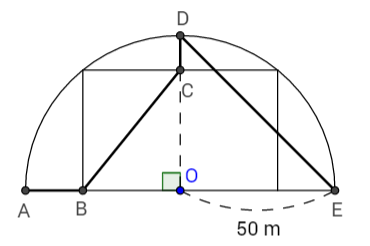
\includegraphics[width=0.5\textwidth]{1}
\end{figure*}
\ans{\(80+50\sqrt2\)}

%
\prob{}
상수가 아닌 두 다항식 \(f(x)\), \(g(x)\)에 대하여 \(f(x)\)를 \(g(x)\)로 나눈 몫을 \(Q(x)\), 나머지를 \(R(x)\)라고 할 때, 옳은 것만을 <보기>에서 있는 대로 고른 것은?
\begin{mdframed}[frametitle=<보기>]
\begin{enumerate}[ㄱ.]
\item
\(f(x)-Q(x)\)를 \(Q(x)\)로 나눈 나머지는 \(R(x)\)이다.\\
(단, (\(R(x)의\:\:차수)<(Q(x)의 차수)\))
\item[ㄴ.]
\(f(x)+Q(x)\)를 \(Q(x)\)로 나눈 나머지는 \(R(x)\)이다.\\
(단, (\(R(x)의\:\:차수)<(Q(x)의 차수)\))
\item[ㄷ.]
\(f(x)\)를 \(Q(x)\)로 나눈 나머지는 \(R(x)\)이다.
\end{enumerate}
\end{mdframed}
\ans{ㄱ, ㄴ}


%
\prob{}
다항식 \(f(x)\)를 \((x-1)^2\)으로 나눈 나머지는 \(x-3\)이고, \(x-2\)로 나눈 나머지는 \(5\)이다.
다항식 \(f(x)\)를 \((x-1)^2(x-2)\)로 나눈 나머지를 구하시오.
\ans{\(6x^2-11x+3\)}

\newpage
%
\prob{}
\(x\)에 대한 다항식 \(f(x)=ax-b\)가 다음 두 조건을 만족시킬 때, \(f(2)\)의 값은?
(단, \(a\), \(b\)는 \(a\neq b\)인 상수이다.)
\begin{mdframed}
\begin{enumerate}[(가)]
\item
\(f(x^3)\)을 \(f(x)\)로 나눈 나머지는 \(8a-b\)이다.
\item[(나)]
\(f(x^4)\)을 \(f(x^2)\)으로 나눈 나머지는 \(4\)이다.
\end{enumerate}
\end{mdframed}

%
\prob{}
다항식 \(f(x)\)에 대하여 \(f(x)-2\), \((x-1)f(x)+6\)이 일차식 \(x-\alpha\)로 나누어 떨어질 때, 상수 \(\alpha\)의 값은?
\ans{\(-2\)}

%%
%\prob{}
%\(x^3\)의 계수가 \(1\)인 삼차식 \(P(x)\)에 대하여
%\[P(1)=1,\quad P(2)=2,\quad P(3)=3\]

%
\prob{}
\(x\)에 대한 이차식 \(f(x)\)가 다음 조건을 만족시킬 때, \(g(3)\)의 값은?
\begin{mdframed}
\begin{enumerate}[(가)]
\item
\(x^3+3x^2+4x+2\)를 \(f(x)\)로 나눈 나머지는 \(g(x)\)이다.
\item[(나)]
\(x^3+3x^2+4x+2\)를 \(g(x)\)로 나눈 나머지는 \(f(x)-x^2-2x-1\)이다.
\end{enumerate}
\end{mdframed}
\ans{\(4\)}

%
\prob{}
\(1000\)개의 이차식
\[f_n(x)=x^2+2x-n\quad(n=1,2,3,\cdots,1000)\]
중에서 계수가 정수인 두 일차식의 곱으로 인수분해되는 \(f_n(x)\)의 개수를 구하시오.
\ans{\(30\)}

%
\prob{}
\(a+b=-1\), \(b+c=-2\),
\[(a+b+c)(bc+ca+ab)-abc=-18\]
일 때, \(a+c\)의 값은?
\ans{\(-9\)}

%
\prob{}
\(x+y+z=3\), \(xy+yz+zx=5\), \(xyz=8\)일 때, \((x+y)(y+z)(z+x)\)의 값은?
\ans{\(7\)}

%
\prob{}
다항식 \(x^4-2(a^2+b^2)x^2+(a^2-b^2)^2\)을 인수분해 하시오.
\ans{\((x+a+b)(x-a-b)(x+a-b)(x-a+b)\)}

%
\prob{}
세 실수 \(a\), \(b\), \(c\)에 대하여
\[a+b+c=0,\qquad a^2+b^2+c^2=9\]
일 때, \(a^2b^2+b^2c^2+c^2a^2\)의 값을 구하시오.
\ans{\(\frac{81}4\)}

%
\prob{}
\(x\)에 대한 이차식 \(f(x)\)가 다음 조건을 만족시킨다.
\begin{mdframed}
\begin{enumerate}[(가)]
\item
\(f(0)=0\)
\item[(나)]
모든 실수 \(x\)에 대하여 \(\{f(x)\}^2=f(x^2)\)이다.
\end{enumerate}
\end{mdframed}
다항식 \(\{f(x)-1\}^3\)의 상수항을 포함한 모든 계수의 합은?
\ans{\(0\)}

%
\prob{}
\(x-y=1\)을 만족시키는 모든 실수 \(x\), \(y\)에 대하여
\[ax^2+bxy+cy^2=3\]
이 성립하도록 상수 \(a\), \(b\), \(c\)의 값을 정할 때,
\(a-b-c\)의 값을 구하시오.
\ans{\(6\)}

%
\prob{}
두 다항식 \(f(x)\), \(g(x)\)에 대하여 \(f(x)+g(x)\)는 \(x+1\)로 나누어떨어지고, \(f(x)-g(x)\)를 \(x+1\)로 나누었을 때의 나머지가 \(4\)이다.
\(x+1\)로 나누어떨어지는 다항식인 것만을 <보기>에서 있는 대로 고른 것은?
\begin{mdframed}[frametitle=<보기>]
\begin{enumerate}[ㄱ.]
\item
\(f(x)+2x\)
\item[ㄴ.]
\(f(x)g(x)\)
\item[ㄷ.]
\(\{f(x)\}^2g(x)-4g(x)\)
\end{enumerate}
\end{mdframed}
\ans{ㄱ, ㄷ}

%
\prob{}
\(x\)에 대한 다항식 \(f(x)\)를 \((x-1)^3\)으로 나누었을 때의 나머지가 \(2x^2-x+7\)이고, 다항식 \(f(x)\)를 \((x-1)^2\)으로 나누었을 때의 나머지가 \(px+q\)일 때, 두 상수 \(p\), \(q\)에 대하여 \(p^2+q^2\)의 값을 구하시오.
\ans{\(34\)}

%
\prob{}
계수가 모두 정수인 일차 이상의 두 다항식 \(f(x)\), \(g(x)\)가 등식 \(f(x)g(x)=x^4-x^3-2x^2+3x-1\)을 만족시킨다.
다항식 \(f(x)+g(x)\) 중에서 차수가 가장 낮은 다항식을 \(F(x)\), 가장 높은 다항식을 \(G(x)\)라고 할 때, \(F(2)-G(2)\)의 값은?
\ans{\(0\)}

%
\prob{}
다항식 \(f(x)=x^3-5x^2+3x+9\)에 대하여 \(f(103)\)의 값은?
\ans{\(1040000\)}

%
\prob{}
모든 실수 \(x\)에 대하여
\[x^4+2x^3-x^2+ax+b=(x^2+px+q)^2\]
이 성립할 때, 두 상수 \(a\), \(b\)의 곱 \(ab\)의 값을 구하시오.
\ans{\(-2\)}

%
\prob{}
복소수 \((i-1)x+2(-3+2i)\)를 제곱하면 음의 실수가 된다고 할 때, 실수 \(x\)의 값을 구하시오.
\ans{\(-6\)}

\newpage
%
\prob{}
\(z\neq0\)인 모든 복소수 \(z\)에 대하여 항상 실수인 것만을 <보기>에서 있는 대로 고른 것은?
\begin{mdframed}[frametitle=<보기>]
\begin{enumerate}[ㄱ.]
\item
\(z+\bar z\)
\item[ㄴ.]
\(z^2-{\bar z}^2\)
\item[ㄷ.]
\(\displaystyle\frac1z+\frac1{\bar z}\)
\end{enumerate}
\end{mdframed}
\ans{ㄱ, ㄷ}

%
\prob{}
두 등식 \(\sqrt{a+1}\sqrt{a-2}=-\sqrt{(a+1)(a-2)}\), \(\displaystyle\frac{\sqrt{-a+3}}{\sqrt{-a-4}}=-\sqrt{\frac{-a+3}{-a-4}}\)을 만족시키는 정수 \(a\)의 개수는?
\ans{\(4\)}

%
\prob{}
\(x\)에 대한 이차방정식 \(x^2-(k+2)x+18=0\)의 한 근이 다른 근의 \(2\)배일 때, 모든 실수 \(k\)의 값의 합은?
\ans{\(-4\)}

%
\prob{}
\(x\)에 대한 이차방정식 \(x^2-(a+3)x+3a+2=0\)의 두 근이 연속된 자연수일 때, 자연수 \(a\)의 값은?
\ans{\(6\)}

%
\prob{}
두 유리수 \(a\), \(b\)에 대하여 이차방정식 \(x^2+ax+b=0\)의 한 근이 \(3+\sqrt2\)일 때, 이차방정식 \(x^2+bx+a=0\)의 두 근을 구하시오.
\ans{\(x=-3\) 또는 \(x=2\)}

%
\prob{}
\(x\)에 대한 이차방정식 \(2x^2+(k-1)x+k-2=0\)이 한 개의 양의 실근과 한 개의 음의 실근을 갖도록 하는 실수 \(k\)의 값의 범위를 구하시오.
\ans{\(k<2\)}

%
\prob{}
이차방정식 \(x^2+x-5=0\)의 두 근을 \(\alpha\), \(\beta\)라고 할 때, \((\alpha^2+2\alpha-1)(\beta^2+2\beta-1)\)의 값을 구하시오.
\ans{\(7\)}

%
\prob{}
이차함수 \(y=x^2+2ax+ak+4k-2b\)의 그래프가 실수 \(k\)의 값에 관계없이 항상 \(x\)축에 접할 때, 두 상수 \(a\), \(b\)의 곱 \(ab\)의 값은?
\ans{\(32\)}

%
\prob{}
이차함수 \(y=x^2-2ax+b\)의 그래프가 \(x\)축에 접하고, 직선 \(y=3x\)와 만나지 않을 때, 실수 \(b\)값의 범위는?
\ans{\(b>\frac9{16}\)}

%
\prob{}
\(x\)에 대한 이차방정식 \(x^2+(2-a)x-4=0\)의 한 근이 \(-2\)와 \(-1\) 사이에 존재하고, 다른 한 근은 \(2\)와 \(3\) 사이에 존재하도록 하는 정수 \(a\)의 값을 구하시오.
\ans{\(3\)}

%
\prob{}
\(x\ge2\)에서 이차함수 \(y=x^2-2kx+1\)의 최솟값이 \(-8\)일 때, 상수 \(k\)의 값은?
\ans{\(3\)}

%
\prob{}
어느 과일 가게에서 포도 한 송이를 \(2000\)원에 판매하면 하루에 \(200\)송이를 팔 수 있다.
가격을 \(100\)원 내릴 때마다 판매량이 \(20\)송이씩 증가한다고 할 때, 하루 총 판매 금액을 최대로 하기 위해서는 포도 한송이의 가격을 얼마로 정해야 하는지 구하시오.
\ans{\(1500\)원}

%
\prob{}
이차함수 \(y=2x^2+(3a+4)x+2-a^2\)의 그래프와 직선 \(y=a^2x-5a\)가 서로 다른 두 점에서 만나고 두 교점의 \(x\)좌표가 절댓값이 같을 때, 상수 \(a\)의 값을 구하시오.
\ans{\(-1\)}

%
\prob{}
\(x\)에 대한 사차방정식 \(2x^4-2kx^2+2k-9=0\)이 서로 다른 두 실근과 서로 다른 두 허근을 갖도록 하는 자연수 \(k\)의 개수를 구하시오.
\ans{\(4\)개}

%
\prob{}
\(x\)에 대한 사차방정식 \(x^4+px^3+4x^2+px+1=0\)의 한 근 \(\alpha\)가 등식 \(\alpha+\frac1{\alpha}=1\)을 만족시킬 때, 상수 \(p\)의 값은?
\ans{\(-3\)}

%
\prob{}
이차방정식 \(x^2-x-3=0\)의 서로 다른 두 실근이 \(x\)에 대한 사차방정식 \(x^4+ax^3+bx^2+cx+d=0\)의 두 중근일 때, 네 상수 \(a\), \(b\), \(c\), \(d\)의 합 \(a+b+c+d\)의 값은?
\ans{\(8\)}

%
\prob{}
삼차방정식 \(x^3=-1\)의 한 허근을 \(\omega\)라고 할 때, <보기>에서 옳은 것만을 있는 대로 고른 것은?
\begin{mdframed}[frametitle=<보기>]
\begin{enumerate}[ㄱ.]
\item
\(\displaystyle\omega-\frac1{{\bar\omega}^2}=1\)
\item[ㄴ.]
\(\omega^2+{\bar\omega}^2=0\)
\item[ㄷ.]
\(\displaystyle\frac1{1-\omega}+\frac1{1-\bar\omega}=1\)
\end{enumerate}
\end{mdframed}
\ans{ㄱ, ㄷ}

%
\prob{}
연립방정식
\(\begin{cases}
kx+y+z=3\\
x+ky+z=3\\
x+y+kz=3\end{cases}\)
의 해가 존재하지 않을 때의 \(k\)의 값을 \(\alpha\), 무수히 많을 때의 \(k\)의 값을 \(\beta\)라고 하자.
\(\alpha+\beta\)의 값을 구하시오.
(단, \(k\)는 실수이다.)
\ans{\(-1\)}

\newpage
%
\prob{}
\(x\)에 대한 이차방정식 \(x^2+(m-5)x+m-3=0\)의 두 근이 모두 정수가 되도록 하는 모든 정수 \(m\)의 값의 합은?
\ans{\(14\)}

%
\prob{}
\(x\), \(y\)에 대한 방정식
\[2x^2-4xy+5y^2-4x-2y+5=0\]
을 만족시키는 두 실수 \(x\), \(y\)가 존재할 때, \(x+y\)의 값을 구하시오.

%
\prob{}
모든 실수 \(x\)에 대하여 부등식 \(a^2x-4a>4x-3\)이 성립할 때, 상수 \(a\)의 값은?
\ans{\(-2\)}

%%
%\prob{}
%길이가 각각 \(x\), \(12-2x\), \(2x+1\)인 세 선분을 이용하여 삼각형을 만들려고 할 때, 가능한 자연수 \(x\)의 개수는?
%\ans{\(1\)개}

%
\prob{}
부등식 \(x^2-4|x|-5>0\)의 해가 부등식 \(2x^2+ax+b>0\)의 해와 서로 같을 때, 두 상수 \(a\), \(b\)의 합 \(a+b\)의 값은?
\ans{\(-50\)}

%
\prob{}
\(x\)에 대한 이차부등식 \(f(x)<0\)의 해가 \(-3<x<3\)일 때, 부등식 \(f(2014-x)\ge0\)의 해는?
\ans{\(x\le2011\) 또는 \(x\ge2017\)}

%
\prob{}
세 변의 길이가 \(x-3\), \(2x-1\), \(2x+3\)인 삼각형이 둔각삼각형이 되기 위한 자연수 \(x\)의 최댓값을 \(M\), 최솟값을 \(m\)이라고 할 때, \(M-m\)의 값을 구하시오.
\ans{\(13\)}
\end{document}